\paragraph{Primary comparison.}
Table~\ref{tab:pathtable} reports flow prediction, attribution accuracy,
and the end-to-end error of the reported summary on the same test demand
paths for both networks. On the 96 Sioux Falls paths, response
supervision lowers the median attribution-column error from $21.18\%$ to
$14.19\%$ (a relative reduction of one third) and the family-boundary
error from $8.74\%$ to $5.75\%$, while both models retain total-flow
errors near $0.03\%$ (medians $0.0322\%$ and $0.0292\%$). Measured
against the demand-change increment rather than total flows, the
endpoint flow-prediction error falls from $5.03\%$ to $3.52\%$ --- the
incremental response that the attributions decompose --- so response
supervision improves both the attribution column and the response field
it integrates; the total-flow columns stay near $0.03\%$ because total
flows are dominated by the unchanged background. The improvement holds
in every active-query group
(Appendix~\ref{supp:learningdetail}). Path-level paired differences
quantify the uncertainty: the median paired column-error difference is
$-5.03$ percentage points with a path-level bootstrap $95\%$ interval of
$[-6.01,-4.48]$ (10,000 resamples), improving 92 of 96 paths; the
paired family-boundary difference has median $-2.06$ with interval
$[-2.76,-1.65]$, improving 90 of 96, with every group's interval
excluding zero and leave-one-path-out medians varying within
$[-5.11,-4.94]$ and $[-2.11,-2.00]$. The system-contribution difference
is secondary and opposite in sign (median $+0.45$, interval
$[0.01,0.74]$; both methods below $3.5\%$), confirming that scalar
completeness and spatial explanation accuracy measure different
properties. The improvement is consistent across all five seeds, with
both median error metrics decreasing for every seed and 80--91 of 96
paths improving per seed (Table~\ref{tab:fiveseed},
Appendix~\ref{supp:learningdetail}). The same-path decomposition of
Eq.~\eqref{eq:coldecompmain} attributes the discrepancy to demand-response
error on every path--query pair (path--query median response and weight
norms $206.5$ and $3.5$ under flow supervision, $147.6$ and $3.3$ under
response supervision).
\begin{table}[t]\centering\footnotesize
\caption{Prediction and spatial-explanation accuracy, and the end-to-end
error of the reported summary, on the same test demand paths (Sioux
Falls: 96 paths, 24 per active-query group; Anaheim: 48 paths). Entries
are medians of path-level values (active queries and seeds averaged
within each path; flow errors additionally averaged over the path's
states). Total flow: relative flow error; incremental: endpoint
flow-change error (percent of the reference increment norm); column:
attribution-column error; family boundary: maximum boundary error over
the query's family as a percentage of the reference family maximum (the
Sioux Falls family is the geometric screenline set; Anaheim uses its
ordered distance family); final summary: total error of the reported
minimum-segment summary (percent of the reference family scale;
tolerance $5\%$ of the learned family maximum); segments: median
reported segment count (distinct direction chains on Sioux
Falls).}\label{tab:pathtable}
\setlength{\tabcolsep}{4.5pt}
\begin{tabular*}{\tblwidth}{@{\extracolsep{\fill}}llcccccc}
\toprule
Network & Method & Total flow (\%) & Incremental (\%) & Column (\%) & Family (\%) & Final summary (\%) & Segments\\
\midrule
Sioux Falls & Flow & 0.032 & 5.03 & 21.18 & 8.74 & 11.35 & 117\\
Sioux Falls & Response & 0.029 & 3.52 & 14.19 & 5.75 & 8.68 & 117\\
\addlinespace
Anaheim & Flow & 0.024 & 2.46 & 1.64 & 0.94 & 4.57 & 9.9\\
Anaheim & Response & 0.019 & 2.03 & 1.31 & 0.78 & 4.55 & 9.9\\
\bottomrule\end{tabular*}\end{table}

\paragraph{Where the flow-only explanation breaks, and what supervision
repairs.}
Figure~\ref{fig:repair} shows one pre-specified case: among the 96 test
paths, the one whose paired family-error improvement is closest to the
median improvement (path 22, six active queries; improvement $48.4$
against the median $49.2$), and within it the query with the largest
flow-only family error, OD $(7,12)$. The panels display the query's
longest projection-direction chain (20 nested boundaries, a geometric
display choice independent of attribution values), the boundary error
against the reference along that chain, and the family-wide worst
boundary on the network. The flow-only model does not merely rescale
the profile: it misplaces the attribution across the corridor, with
errors concentrated where the reference profile varies. At the worst
flow-only boundary ($369.5$ TSTT units, on a reference value of
$5{,}619.3$ that is congestion-dominated: $5{,}018.7$ of it from
congestion weights against $600.6$ from free-flow weights) the error
falls to $80.1$ under response supervision --- a $78\%$ reduction at
that boundary; over the whole family, the worst error falls from
$369.5$ to $115.2$ and the end-to-end error of the reported summary
from $679.1$ to $463.7$ at essentially unchanged segment count ($186$
to $190$ over the family). All quantities come from the same
five-seed-median columns the figure displays. The segment summaries of
all three columns sit inside their stated tolerance bands, so the
repair acts on the profile the summaries compress, not on the
compression itself.
\begin{figure}[t]
\centering
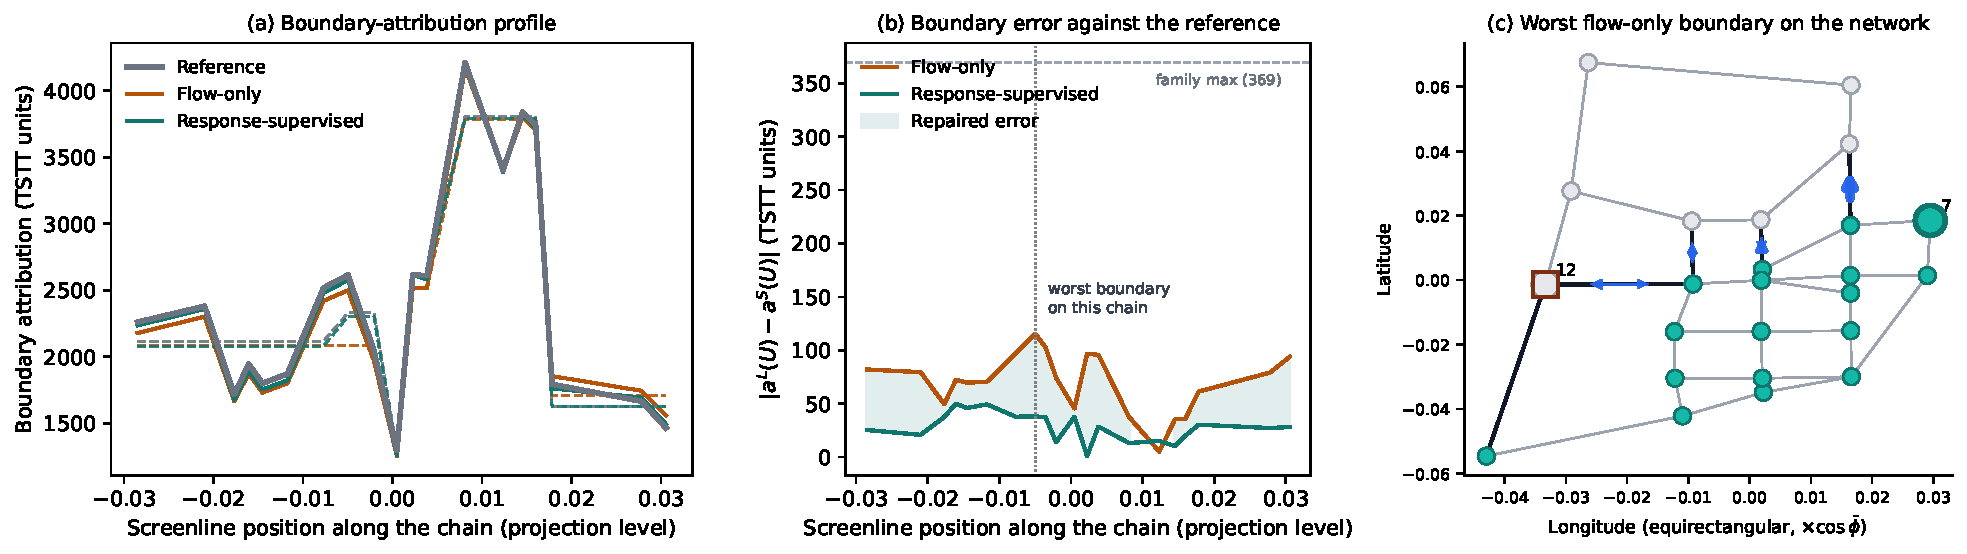
\includegraphics[width=\linewidth]{../figures/fig_v111_repair.pdf}
\caption{A learned spatial profile repaired by response supervision
(pre-specified case: path 22, query $(7,12)$; five-seed median columns).
(a)~Boundary-attribution profile along the query's longest
projection-direction chain (20 nested boundaries at the $10^\circ$
direction): reference (grey), flow-only (ochre), response-supervised
(teal), each with its minimum-segment summary (dashed). (b)~Boundary
error against the reference along the same chain; the dotted line marks
the worst boundary on the chain and the grey dashed line the
family-wide maximum ($369.5$). (c)~The family-wide worst flow-only
boundary on the network: teal nodes form $U$ (origin $7$ ringed,
destination $12$ square); arrow width scales with the signed
crossing-link contribution (solid blue positive, dashed red
negative).}\label{fig:repair}
\end{figure}

\paragraph{The objective family.}
The boundary-error representation of
Eq.~\eqref{eq:localboundarybound} defines a family of supervision
objectives rather than a single loss. Three of its members organize the
comparison: ordinary flow supervision; response supervision, the
unweighted form of Eq.~\eqref{eq:learningobjective}; and
weighted-response supervision, the direct form identified by the
decomposition of Eq.~\eqref{eq:coldecompmain}. Under a shared
continuation budget and a common validation-only weight search
(Appendix~\ref{app:pairs-v102}), the unweighted form attains the lowest
errors on every metric (column $14.19\%$, family boundary $5.75\%$,
flow $0.029\%$) and the widest usable weight range, while the weighted
form reaches $15.21\%$ at its selected weight and improves 84 of 96
paths --- confirming directly that the weight-shift term the unweighted
objective ignores is small. One structural insight separates the
response family from boundary-value losses: $\mathcal K_j$ is a
seminorm whose kernel contains the circulation directions, so
optimizing the boundary value alone cannot restore the response field
that the profile integrates --- the boundary-seminorm objective attains
the lowest validation boundary error yet a test column error above
flow-only training ($24.18\%$, improving only 8 of 96 paths), whereas
supervising the response field improves every spatial error metric.
The complete six-objective comparison, including the endpoint
objectives, the weight grids and the explanation--flow frontier,
appears in Appendix~\ref{app:legacy-learning} (Table~\ref{tab:fairmethods},
Figure~\ref{fig:v109pareto}).

\paragraph{Label efficiency.}
Retraining response supervision at the selected weight with per-query
derivative-center budgets of $6$, $12$, $24$ and $48$ (36--288 centers
in total; the full budget is 384), each with three independent
query-balanced random nested subsets, shows the improvement emerging
quickly and robustly (Figure~\ref{fig:v109labelbudget},
Appendix~\ref{app:labelbudget}): the median
column error falls to $16.35\%$ at 36 centers and $14.53\%$ at 288,
with subset interquartile ranges of at most $0.8$ percentage points at
every budget, and flow accuracy stays within $0.027$--$0.031\%$
throughout (aggregation and the full-budget point as in
Appendix~\ref{app:labelbudget}). Half of the full column-error improvement is reached with
36 centers, $80\%$ with 144, and $90\%$ with 288; for the
family-boundary error, $80\%$ is reached already at 72 centers. Each
training center costs one reference flow solve and one sensitivity
solve, so response supervision showed favourable label efficiency in
the studied setting.
\paragraph{Training budget and wall-clock.}
Neither method sits at a validation plateau at the 1{,}200-update cap,
and response supervision exhibits persistent anytime dominance under
the shared protocol: repeating the continuation with the budget
tripled to 3{,}600 updates under the identical initialization,
learning rate, batches, label sets and selection rule
(Figure~\ref{fig:v109convergence}, Appendix~\ref{supp:learningdetail})
improves both objectives on both networks while the response curve
stays below the flow curve throughout. On the 96 test paths, flow-only
training improves its median column error from $21.18\%$ to $19.46\%$
and response supervision from $14.19\%$ to $11.41\%$; on Anaheim's 48
paths, from $1.64\%$ to $1.24\%$ and from $1.31\%$ to $0.88\%$; the
column-error ratio falls from $0.67$ to $0.59$ on Sioux Falls and from
$0.80$ to $0.71$ on Anaheim. Derivative supervision costs more per
update ($1.8\times$ on Sioux Falls, $3.3\times$ on Anaheim under the
shared CPU protocol). In wall-clock terms the picture differs by
network. On Sioux Falls the dominance survives the cost difference: at
the flow method's total training time, the response-supervised
validation boundary error is already three times lower. On Anaheim the
larger per-update cost delays the crossover: at the flow method's
total training time the response run has not yet caught up, and it
reaches the flow method's final error only after about $2.2$ times
that budget (after which it continues to improve while the flow run
has stopped). The equal-update dominance therefore carries a
wall-clock overhead on Anaheim, and the reported operating points
remain budget-limited with the larger remaining headroom on the
response method.

\paragraph{End-to-end explanation error.}
The quantities of Table~\ref{tab:pathtable} concern the learned
profiles; the reported artifact is the learned model's minimum-segment
summary, whose total error Table~\ref{tab:pathtable} already carries as
the budget of Eq.~\eqref{eq:totalbudget} at the working $5\%$ tolerance.
Figure~\ref{fig:v110resolution} traces the same quantities as the
tolerance --- and with it the number of reported segments --- varies
from $0.5\%$ to $10\%$: the x axis is the number of segments a reader
must absorb, the y axis the final error of the reported summary against
the reference explanation. The two networks occupy different regimes,
and the error budget identifies the effective lever on each. On Sioux
Falls the model term dominates ($8.74\%$ against a $4.76\%$ summary
term under flow supervision), the response-supervised curve lies
strictly below the flow-supervised curve at every segment count, and a
final error of $11.5\%$ needs 77 segments under response supervision
but 117 under flow supervision --- or, at the same 117 segments,
response supervision lowers the final error from $11.35\%$ to
$8.68\%$. On Anaheim the learned columns are closer to the reference,
and at the working $5\%$ tolerance the budget is compression-dominated:
the summary term ($4.3\%$) is several times the model term ($0.9\%$),
the two methods yield nearly the same total error, and both curves
track the reference-compression curve --- the error of compressing the
reference profile itself at each tolerance, plotted at its own segment
count. At the tightest $0.5\%$ tolerance the model term takes over
($0.9\%$ and $0.8\%$ against a $0.5\%$ summary term), so tightening
further there requires a better learned response. The relative
importance of model and compression errors therefore differs across
networks and tolerances, and the error budget identifies whether
improving the learned response or refining the spatial summary is the
more effective route to a more accurate explanation. On both networks
the measured total error of the reported summary stays within the
budget on every path. Relative to the baselines, segmentation cuts the
total error by a factor of $3.0$--$3.8$ (single common value) and
$1.7$--$2.0$ (equal-count) on Sioux Falls, and by $10.5$--$10.6$ and
$10.2$ on Anaheim --- where the strongly ordered profiles make
equal-count segmentation nearly as coarse as a single value, so
position-aware segmentation is what carries the error control; the
paired total error improves on $93.1\%$ of Sioux Falls path--query
pairs under response supervision. The final-summary entries of
Table~\ref{tab:pathtable} are medians of budget components computed on
each path--query--seed before aggregation, so they do not add to a
guarantee for any single explanation.
\begin{figure}[t]
\centering
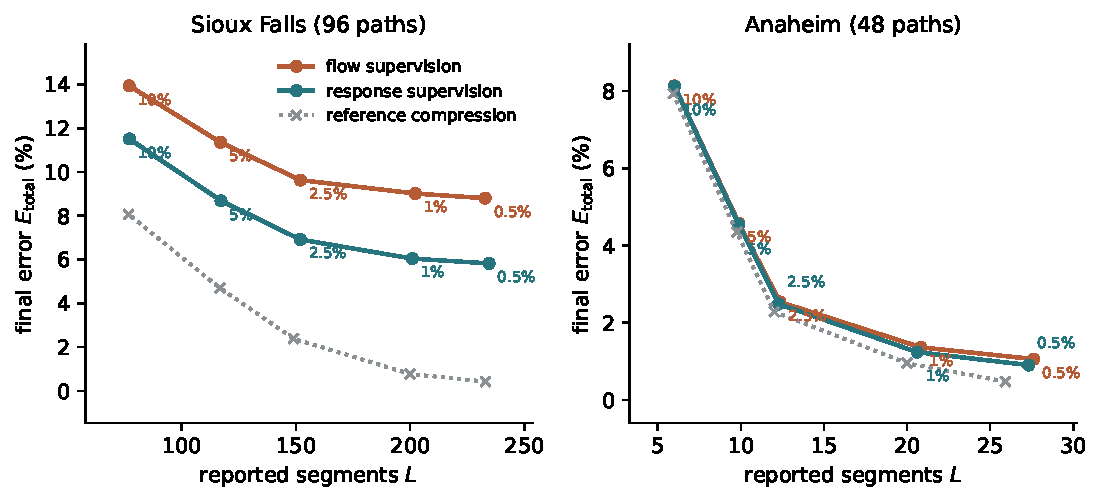
\includegraphics[width=\linewidth]{../figures/fig_v110_resolution.pdf}
\caption{Final error of the reported summary against the number of
reported segments, as the family tolerance varies over $0.5$--$10\%$
(annotated; percent of the learned family maximum). Sioux Falls
(left): model-error dominated --- the response-supervised curve (teal)
lies below the flow-supervised curve (ochre) at every segment count, so
better responses convert into either fewer segments at equal accuracy
or more accurate summaries at equal complexity. Anaheim (right):
compression dominated at the working tolerance --- both curves track
the grey reference-compression curve, the error of compressing the
reference profile itself at each tolerance, plotted at its own segment
count ($\times$ marks). Per-tolerance segmentation recomputed from the
final learned profiles; common per-query normalization as in
Table~\ref{tab:pathtable}.}\label{fig:v110resolution}
\end{figure}

\paragraph{Bound tightness.}
Computed with the same $41$-state trapezoidal quadrature for both
sides, the exact unrestricted errors $\mathcal K_j(e_j)$ lie below the
integrated bounds $B_j$ of Eq.~\eqref{eq:localboundarybound} (the
numerical verification and quadrature accuracy are reported in
Appendix~\ref{supp:accuracy}). The chain is tight: the median ratio
$\mathcal K_j(e_j)/B_j$ is $0.95$ for flow supervision (quartiles
$0.91$--$0.98$) and $0.95$ for response supervision (quartiles
$0.90$--$0.97$). The integrated bound is therefore a tight
\emph{a posteriori} upper bound on the realized worst boundary error
--- it uses reference-response information, as
Section~\ref{sec:totalbudget} notes --- and response supervision lowers
the family, unrestricted and bound levels in parallel. The geometric
family retains about half of the unrestricted error (median ratio
$E^{\mathrm{geo}}/\mathcal K_j(e_j)$ $0.51$ and $0.48$), so the
single-family errors reported throughout should be read as lower
bounds on the worst separating-region error.
